%====================================================================================
\section[Tobit]{El modelo Tobit para las respuestas de la solución Corner}
%====================================================================================
\subsection{Motivación}
\begin{frame}[fragile]
	\frametitle{Motivación}
	
	\begin{enumerate}
		\item Ejemplo 1: En una encuesta de hogares se observa el salario solo de aquellos que trabajan, el resto de sus características son conocidas (sexo, edad, etc) 
		
		\item Ejemplo 2: Se encuesta a mujeres que trabajan.
		
		\item Ejemplo 3: Los resultados de una encuesta televisada son representativos de todos los votantes?.
		
	\end{enumerate}
	
	%Si la variable dependiente es el salario, en el primer caso esta es observada para aquellos que trabajan, los covariados (otras características) si son observadas. En el segundo caso la variable dependiente y covariados no son observados para los que no trabajan. 
	
\end{frame}

\subsection{Algunas propiedades}

\begin{frame}[fragile]
	\frametitle{Propiedades distribución normal}
	
	\begin{eqnarray*}
		f(x) &=& \frac{1}{\sqrt{2\pi\sigma^2}} exp \left[ -\frac{(x-\mu)^2}{2\sigma^2}
		\right] \\
		\phi(z) &=& \frac{1}{\sqrt{2\pi}} exp \left[ -\frac{(z)^2}{2} \right]
	\end{eqnarray*}
	
	\begin{itemize}
		\item $\phi(-z)=\phi(z)$
		\pause
		\item $\frac{\partial \phi(z)}{\partial z}=-z \phi(z)$
		\pause
		\item $f(x)=\frac{1}{\sigma} \phi \left[ \frac{x-\mu}{\sigma} \right]
		\pause
		= \frac{1}{\sigma} \phi (z)$
		\pause
		\item $\Phi(a)=P(z<a)=\int_{-\infty}^{a}\phi(z)dz$
		\pause
		\item $\Phi(-a)=1-\Phi(a)=P(z\geq a)$
	\end{itemize}
	
\end{frame}

\begin{frame}[fragile]
	\frametitle{Distribución truncada}
	\begin{itemize}
		\item $f(x|x>a)=\frac{f(x)}{P(x>a)}$
		\item $E(x|x>a)>E(x)$
		\item $Var(x|x>a)<Var(x)$
	\end{itemize}
\end{frame}

\begin{frame}[fragile]
	\frametitle{Distribución normal truncada}
	
	Sea $x$ una variable aleatoria distribuida normalmente: $x \sim
	N(\mu,\sigma^2)$, entonces:
	
	\begin{itemize}
		\item $\lambda(\alpha)=\frac{\phi(\alpha)}{1-\Phi(\alpha)}$ donde
		$\alpha=\frac{a-\mu}{\sigma}$. Evaluar y graficar en $\alpha=0$
		\item $\delta(\alpha)=\lambda(\alpha)[\lambda(\alpha)-\alpha]$
		\item $0<\delta(\alpha)<1$
		\item $\lambda(\alpha)$ es conocido como el inverso del ratio de Mills.
		\item $E(x|x>a)=\mu+\sigma\lambda(\alpha)$
		\item $Var(x|x>a)=\sigma^2[1-\delta(\alpha)]$
	\end{itemize}
\end{frame}

\subsection{El modelo de regresión truncado}

\subsubsection{Definición}

\begin{frame}[fragile]
	\frametitle{Caso: Promedio truncado NO condicionado}
	
	Por medio de una encuesta a empresas formales sólo los trabajadores con ingresos
	superiores a S/.930 son declarados. Si se estima que el
	porcentaje de trabajadores con un sueldo superior a S/.930 es el
	80$\%$ de los trabajadores, y que el salario promedio de los
	entrevistados es de S/.1,800 Nuevos Soles. Estime el salario promedio
	de todos los trabajadores. 
	\bigskip
	
	\emph{\textbf{Solución:}}
	\pause
	\begin{eqnarray}
		E(x|x>930) &=& \mu+\sigma\frac{\phi[(930-\mu)/\sigma]}{1-\Phi} \\
		\Phi(\alpha) &=& 20\%; \alpha=(930-\mu)/\sigma
	\end{eqnarray}
	
	Ayuda, utilice los comandos -\texttt{invnormal}- y -\texttt{normalden}-
\end{frame}

\begin{frame}[fragile]
	\frametitle{El modelo de regresión truncado}
	
	La muestra está sistemáticamente restringida a solo una parte de
	la población. Por ejemplo, una muestra puede solo incluir personas
	que están empleadas, o gente sobre una cierta edad.
	\bigskip
	\pause
	
	$Y_i=X_i\beta+\mu_i$; $\mu_i \sim N(0,\sigma^2)$ \\
	\medskip
	
	\pause
	
	$Y_i|X_i \sim N[X_i \beta,\sigma^2]$ \\
	\smallskip
	
	\pause
	
	$$E[y_i|y_i>a]=X_i\beta+\sigma\frac{\phi(\alpha_i)}{1-\Phi(\alpha_i)}$$
	\smallskip
	
	donde:
	\medskip
	
	\pause
	$\alpha_i=\frac{a-X_i\beta}{\sigma}$ y $\phi$ y
	$\Phi$ son las funciones de densidad y acumulada de una variable
	aleatoria normal estándar. \\
	\smallskip
	
	\pause
	
	$$E[y_i|y_i>a]=X_i\beta+\sigma\lambda(\alpha_i)$$
	
\end{frame}

\begin{frame}
	El modelo a estimar sería entonces:
	$$y_i=X_i\beta+\sigma \lambda(\alpha_i)+\varepsilon_i$$
	
	Donde $\alpha_i=\frac{a-X_i\beta}{\sigma}$
	
	\bigskip
	
	Así, si se estima el modelo sin incorporar $\lambda$ se tendría un problema de variable omitida los parámetros serían sesgados e inconsistentes.
	
\end{frame}

\begin{frame}
	\frametitle{Regresión truncada versus MCO}
	\begin{figure}
		\centering
		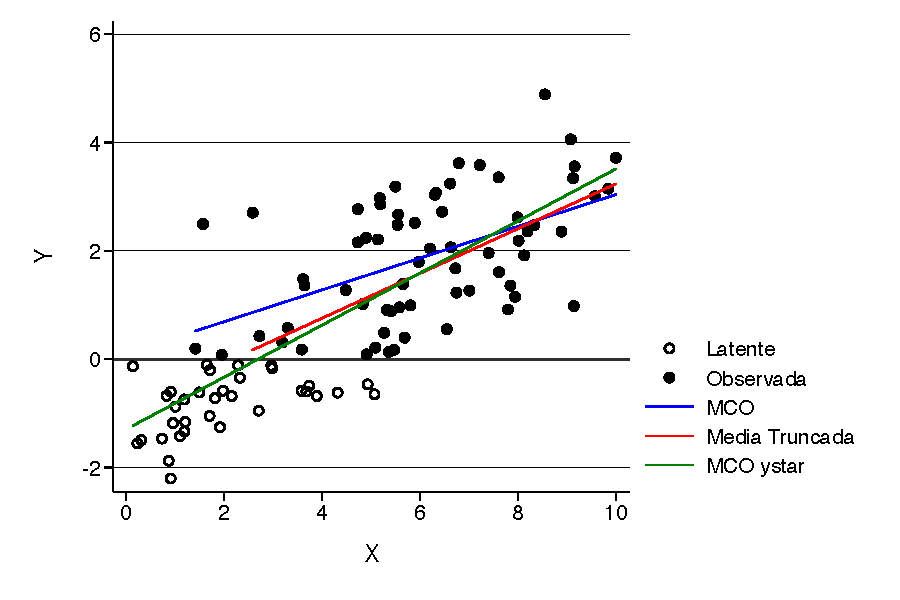
\includegraphics[scale=.75]{fig/truncreg.pdf}
	\end{figure}
\end{frame}


\subsubsection{Efectos marginales}

\begin{frame}
	\frametitle{Efectos marginales}
	
	\begin{itemize}
		\item La interpretación de los parámetros dependen de la pregunta de
		investigación. 
		\item Si el investigador esta interesado en la relación entre las variables 
		para la población entera, los coeficientes $\beta$ son interpretados como los efectos marginales. 
		\item Sin embargo, si el interés en el efecto en la submuestra, el efecto marginal se estima de la siguiente manera:
		
		
		$$\frac{\partial E[y_i|y_1>a]}{\partial X}=\beta+\sigma
		\frac{\partial \lambda}{\partial \alpha}\frac{\partial
			\alpha}{\partial X}=\beta(1-\delta(\alpha))$$
		
		\item Es decir, el efecto marginal es inferior que $\beta$, pues $0<\delta(\alpha)<1$.
	\end{itemize}
	
\end{frame}

\subsubsection{Estimación}

\begin{frame}
	\frametitle{Estimación}
	
	\begin{eqnarray*}
		ln \ell &=& \sum_{i=1}^{N} ln \left[ \sigma^{-1} \phi \left(  \frac{y_i-x_i'\beta}{\sigma} \right)  \right]-
		\sum_{i=1}^{N} ln \left[1-\Phi \left( \frac{a-x_i'\beta}{\sigma} \right)  \right]
	\end{eqnarray*}
\end{frame}


\subsection{El modelo de regresión censurado}

\subsubsection{Definición}

\begin{frame}
	\frametitle{El modelo de regresión censurado}
	\begin{itemize}
		\item Un modelo es censurado cuando los valores
		de la variable dependiente se encuentran restringidos a un rango
		de valores. 
		\item La diferencia con el truncamiento es que mientras en
		este modelo sólo se observa una submuestra, en censura se tiene
		información de las variables independientes de toda la muestra.
		\item Dos ejemplos famosos por el uso de esta metodología son los
		realizados por Tobin (1958) y por Fair (1978). 
		\item El primero estudió los determinantes del gasto en bienes durables (dichos gastos se
		acumulan en 0 y luego tienen valores positivos), mientras que el
		segundo estudió el número de relaciones
		extramaritales\footnote{Aunque Fair usó un modelo tipo Tobit se
			puede argumentar que un modelo tipo \emph{``Count Data''} es más
			apropiado.} .
	\end{itemize}
\end{frame}

\begin{frame}
	\frametitle{El modelo (Tobit tipo 1)}
	Considere un modelo estándar probit basado en la decisión de
	comprar algo. Sea $y^*$ una variable índice o latente que se asume
	puede ser modelado como:
	
	\begin{center}
		$y_i^* = x_i'\beta+\epsilon_i $  donde   $ \epsilon_i \sim N(0,\sigma^2)$
	\end{center}
	
	Lo que determina:
	
	\begin{itemize}
		\item $y_i=1$ si $y_i^*>0$
		\item $y_i=0 $ si $y_i^* <= 0$
	\end{itemize}
	
	Si además de conocer si el individuo compra o no, se conoce lo
	gastado en la compra, se tendría el modelo conocido como
	Tobit\footnote{El nombre es en honor de Tobin, quién en 1958 fue
		el primero que lo propuso}:
	
	\begin{itemize}
		\item $y_i=y_i^*$ si $y_i^*>0$
		\item $y_i=0 $ si $y_i^* <= 0$
	\end{itemize}
\end{frame}

\begin{frame}
	\frametitle{El modelo (Tobit tipo 1)}
	Resumen de lo anterior es:
	$$y_i=max(0,x_i'\beta)$$
	
	\begin{eqnarray*}
		E(y_i|x_i) &=& 0 \cdot P(y_i^* \leq 0 | x_i) + E(y_i^*|y_i^*>0, x_i) \cdot P(y_i^*>0|x_i) \\
		&=& E(y_i^*|y_i^*>0, x_i) \cdot P(y_i^*>0|x_i) \\
		&=& (\mu+\sigma \lambda) \cdot P(x_i'\beta+\epsilon_i>0|x_i) \\
		&=& (x_i'\beta+\sigma\frac{\phi(x_i'\beta/\sigma)}{\Phi(x_i'\beta/\sigma)}) \cdot P(\epsilon_i/\sigma>-x_i'\beta/\sigma|x_i) \\
		&=& (x_i'\beta+\sigma\frac{\phi(x_i'\beta/\sigma)}{\Phi(x_i'\beta/\sigma)}) \cdot \Phi(x_i'\beta/\sigma) \\
		&=&  x_i'\beta \Phi(x_i'\beta/\sigma)+\sigma \phi(x_i'\beta/\sigma)
	\end{eqnarray*}
	
\end{frame}

\subsubsection{Efectos marginales}
\begin{frame}
	\frametitle{Interpretación de los parámetros}
	
	\begin{itemize}
		\item Dependen si estamos interesados en saber algo sobre la media en la
		distribución censurada o los coeficientes del modelo latente. 
		%\item Por ejemplo, si tomamos el caso de los salarios de reserva, debemos
		%preguntarnos si queremos estimar el cambio en las ganancias y en
		%la educación (sea $x_j$) para solo los que trabajan (muestra
		%censurada) o bien la relación entre educación y ganancias
		%(esperadas) para toda la oferta de trabajo.
	\end{itemize}
	
	\begin{itemize}
		\item $\frac{\partial E(y_i| y_i>0,x_i)}{\partial x_j}=\beta_j\left[1-\lambda \left( \frac{x_i\beta}{\sigma}\right)\left[ \frac{x_i\beta}{\sigma} +\lambda\left( \frac{x_i\beta}{\sigma}\right)\right]\right]<\beta_j$
		\item $\frac{\partial E(y_i| x_i)}{\partial x_j}=\beta_j \Phi(\frac{x_i\beta}{\sigma})<\beta_j$
		\item  $\frac{\partial E(y_i^*|x)}{\partial
			x_j}=\beta_j$
	\end{itemize}
	
\end{frame}

\begin{frame}
	\frametitle{El modelo (Tobit tipo 1)}
	
	%En la figura se muestra un ejemplo con distintos modelos para un
	%$N=60$, $K=2$ (una constante con una variable independiente), con
	%un error siguiendo una distribución normal estándar, una variable
	%independiente siguiendo una distribución uniforme y con los
	%parámetros $\beta=(-2; 0,5)'$ y $\sigma=1$.
	
	\begin{figure}
		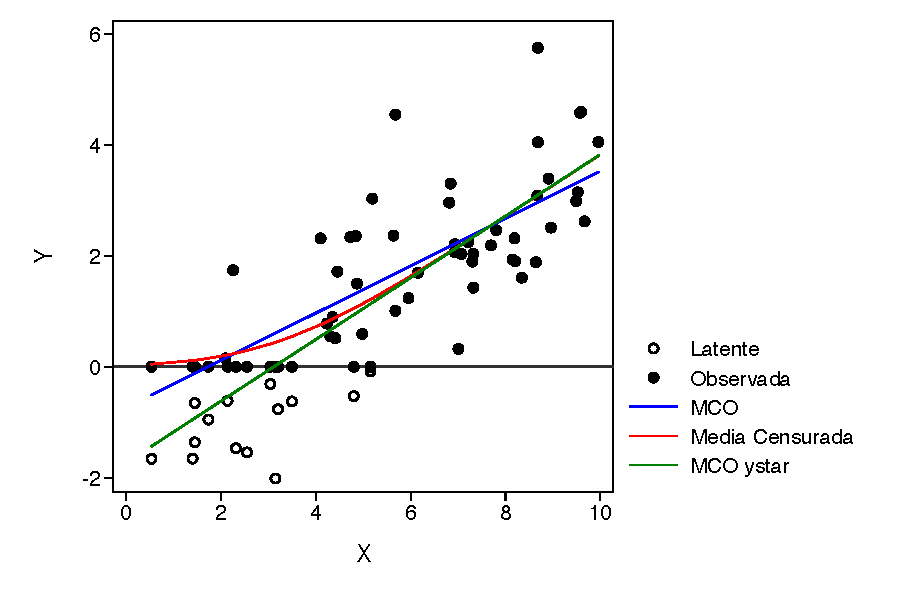
\includegraphics[scale=0.75]{fig/cenreg.pdf}
		%  \caption{Modelo estándar Tobit (Tipo 1)}
	\end{figure}
\end{frame}

\subsubsection{Estimación}

\begin{frame}
	\frametitle{Estimación}
	
	\begin{itemize}
		\item  La estimación MCO de la variable observada $y_i$ sobre $x_i$
		$y_i=x_i'\beta+\mu_i$ produce estimadores sesgados de $\beta$,
		pues $E(y_i|x_i)=x_i'\beta\Phi(x_i'\beta/\sigma)+\sigma
		\phi(x_i'\beta/\sigma)$ no es una función lineal de $x_i$. 
		\item Incluso restringir la muestra a las observaciones que son observadas
		($y_i>0$) no resuelven el problema, pues como se sabe la
		especificación de la regresión truncada es
		$E(y_i|y_i>0,x_i)=x_i'\beta+ \sigma\lambda(x_i'\beta/\sigma)$, es
		decir, de estimar el modelo sin incluir $\lambda$ se tendría un
		problema de variable omitida.
	\end{itemize}
	
\end{frame}

\begin{frame}
	\frametitle{Estimación}
	
	\begin{itemize}
		\item  Asumiendo independencia entre observaciones, el modelo Tobit es
		usualmente estimado por MV, siendo necesario entonces definir la
		función de verosimilitud. 
		\item A diferencia de la función de densidad de una distribución truncada, que es escalada por el término $1/(1-\Phi(\alpha))$ para que la masa de probabilidad siga siendo
		igual a 1, en el caso censurado la función de densidad es una
		combinación de dos funciones, una discreta y otra continua. 
		\item La discreta es donde se acumulan los puntos luego del truncamiento (0
		por ejemplo) y la continua es la función de densidad convencional.
	\end{itemize}
	
\end{frame}

\begin{frame}
	\frametitle{Estimación}
	
	\begin{eqnarray*}
		Prob(y_i=0) &=& Prob(y^*_i \leq 0)=Prob(-x_i'\beta \geq \epsilon_i) \\
		&=& Prob(-x_i'\beta/\sigma \geq \epsilon_i/\sigma) \\
		&=& 1-\Phi(\frac{x_i'\beta}{\sigma}) \\
		Prob(y_i=y_i^*) &=& Prob(y_i=x_i'\beta+\epsilon_i)=Prob(\epsilon_i=y_i-x_i'\beta)  \\
		&=& f(y_i-x_i'\beta) \\
		&=& \frac{1}{\sigma}\phi((y_i-x_i'\beta)/\sigma)
	\end{eqnarray*}
	
\end{frame}

\begin{frame}
	\frametitle{Estimación}
	
	Con lo cual, la función de verosimilitud queda definido como:
	
	\begin{eqnarray*}
		\ell &=& \Pi_{y_i=0}\left[1-\Phi\left( \frac{x_i'\beta}{\sigma} \right)
		\right] \cdot \Pi_{y_i=y_i^*}\left[\frac{1}{\sigma}\phi\left(\frac{y_i-x_i'\beta}{\sigma}\right)\right]
	\end{eqnarray*}
	
	y la función log-l:
	
	\begin{eqnarray*}
		ln \ell &=& \sum_{y_i=0}\left[1-\Phi\left( \frac{x_i'\beta}{\sigma} \right)
		\right] + \sum_{y_i=y_i^*} \left[ -\frac{1}{2} ln(2 \pi)+ln(\sigma^2) +
		\frac{(y_i-x_i'\beta)^2}{\sigma^2} \right]
	\end{eqnarray*}
	
\end{frame}

\subsection{Modelo de Heckman (Heckit)}
\begin{frame}[fragile]
	\frametitle{Modelo de Heckman}
	
	\begin{eqnarray}
		y_{1i} &=& x_{1i}\beta_1+\mu_{1i} \quad \mbox{(Ecuación de regresión)} \\
		y_{2i}^* &=& x_{2i}\beta_2+\mu_{2i} \quad \mbox{(Ecuación de selección)} \\
		y_{2i} &=& 1[y_{2i}^*>0] \quad \mbox{(Dicotómica de selección)} 
	\end{eqnarray}
	
\end{frame}

\begin{frame}[fragile]
	\frametitle{Modelo de Heckman}
	
	Por ejemplo:
	
	\begin{enumerate}
		\item Regresión: Ecuación de salarios, donde $x_1$ son los determinantes de la productividad.
		\item Selección: Decisión de trabajar, donde $y_{2}^*$ puede ser leído como la utilidad neta del trabajo y $x_2$ son los determinantes de la decisión de trabajar.
		\item Dicotómica que clasifica a las personas según estas trabajen o no (ocurre cuando $y_{2}^*>0$)
	\end{enumerate}
	
\end{frame}

\subsection{Supuestos}

\begin{frame}[fragile]
	\frametitle{Modelo de Heckman}
	\begin{enumerate}
		\item $(y_{2i}, x_{2i})$ información disponible para todos.
		\item $(y_{1i}, x_{1i})$ información disponible solo si $y_{2i}=1$ (muestra bajo selección).
		\item $(\mu_{1i}, \mu_{2i})$ independientes de $x_{2i}$, con esperanzas nulas.
		\item $\mu_{2i} \sim N(0,\sigma_2^2)$
		\item $E(\mu_{1i} | \mu_{2i})=\gamma \mu_{2i}$
	\end{enumerate}
	
	Donde la ecuación $(5)$ es la que determina que el modelo sea de selección y no una regresión ordinaria.
	
\end{frame}

\subsection{Problema}

\begin{frame}[fragile]
	\frametitle{Modelo de Heckman: Problema}
	
	%\begin{eqnarray*}
	%y_{1i} = x_{1i}\beta_1+\mu_{1i}
	%\end{eqnarray*}
	%la variable de selección es que las personas trabajan o no trabajan.
	
	\begin{eqnarray}
		E(y_{1i}|x_{1i},y_{2i}=1) &=& x_{1i}\beta_1+E(\mu_{1i}|x_{1i},y_{2i}=1)  \\
		&=& x_{1i}\beta_1+E( E(\mu_{1i} | \mu_{2i})| x_{1i},y_{2i}=1) \\
		&=& x_{1i}\beta_1+E( \gamma \mu_{2i} | x_{1i},y_{2i}=1) \\
		&=& x_{1i}\beta_1+ \gamma E( \mu_{2i} | x_{1i},y_{2i}^*>0) \\
		&=& x_{1i}\beta_1+ \gamma E( \mu_{2i} | x_{1i},\mu_{2i}^*>-x_{2i}\beta_2) \\
		&=& x_{1i}\beta_1+ \gamma [E( \mu_{2i}  + \sigma_2 \lambda(-x_{2i}\beta_2/\sigma_2)] 	 \\
		&=& x_{1i}\beta_1+ \gamma  \sigma_2 [ \lambda(-x_{2i}\beta_2/\sigma_2)] 	\\ 
		&=& x_{1i}\beta_1+ \gamma  \sigma_2 z_i \not=x_{1i}\beta_1 	 
	\end{eqnarray}
	Problema: Estimar  MCO con la muestra bajo selección es inconsistente.
\end{frame}

\subsection{Solución}

\begin{frame}[fragile]
	\frametitle{Modelo de Heckman: Solución 1/4}
	
	\begin{itemize}
		\item Heckman (1979) estudió el sesgo de selección como un problema de especificación incorrecta.
		\item En este caso la variable omitida $z_i$ genera inconsistencia.
		\item Donde la fuente de la inconsistencia es la correlación entre $\mu_{1i}$ y $\mu_{2i}$.
		\item En particular que en $E(\mu_{1i} | \mu_{2i})=\gamma \mu_{2i}$, $\gamma \not = 0$
		\item La gran contribución de Heckman fue notar que el sesgo de selección es un sesgo por omisión de variables.
		\item La fuente de la selección es la correlación entre el mecanismo de selección y la regresión a través de sus errores.
		\item Usando LEI, se puede probar que $E(\mu_1,\mu_2)=\gamma \sigma_2^2$
	\end{itemize}
	
\end{frame}
%---------------------------------------------------
\begin{frame}[fragile]
	\frametitle{Modelo de Heckman: Solución 2/4}
	
	\begin{eqnarray}
		E(y_{1i}|x_{1i},y_{2i}=1) = x_{1i}\beta_1+\gamma \sigma_2 z_i \\
		y_{1i} = x_{1i}\beta_1+\gamma \sigma_2 z_i + \mu_{1i}^*
	\end{eqnarray}
	
	\begin{itemize}
		\item Si $x_{1i}$ , $z_i$ fuesen observables cuando $y_{2i}=1$; se puede estimar (13) por MCO.
		\item El problema es que $z_i= \lambda(-x_{2i}\beta_2/\sigma_2)$ no es observable, pues $\beta_2$ y $\sigma_2$ no son conocidos.
		\item No es necesario conocer los valores de dichos parámetros por separado, con estimar $\delta=\beta_2/\sigma_2$ es suficiente como para tener un estimador de $z_i$.
	\end{itemize}
	
\end{frame}
%---------------------------------------------------
\begin{frame}[fragile]
	\frametitle{Modelo de Heckman: Solución 3/4}
	
	Se puede estimar $\delta$ usando un probit:
	
	\begin{eqnarray}
		P(y_{2i}=1) &=& P(y_{2i}^*>0)= P(x_{2i}\beta_2+\mu_{2i}>0)  \\
		&=& P(\mu_{2i}> -x_{2i}\beta_2) \\
		&=& P(\frac{\mu_{2i}}{\sigma_2}>- \frac{x_{2i}\beta_2}{\sigma_2}) \\
		&=& P(\frac{\mu_{2i}}{\sigma_2}>- \frac{x_{2i}\beta_2}{\sigma_2}) \\                       	                       			  &=& P(\frac{\mu_{2i}}{\sigma_2}< \frac{x_{2i}\beta_2}{\sigma_2})  \\
		&=& \Phi(x_{2i}\delta)                 
	\end{eqnarray}
	$x_{2i}$ y $y_{2i}$ se observan para todas las personas, $\delta$ se puede estimar por MV. No se puede identificar por separado $\beta_2$ y $\sigma_2$
\end{frame}
%---------------------------------------------------
\begin{frame}[fragile]
	\frametitle{Modelo de Heckman: Solución 4/4}
	
	Método en dos etapas 
	
	\begin{itemize}
		\item Etapa 1: Estimar $\hat\delta$ usando un probit.
		
		$$P(y_{2i}=1)=\Phi(x_{2i}\delta)$$
		
		Se usa toda la muestra para obtener:
		
		$$z_i= \lambda(\frac{-x_{2i}\beta_2}{\sigma_2})$$
		
		\item Etapa 2: Realizar la regresión de $y_{1i}$ en $x_{1i}$ y $\hat z_i$ usando la muestra bajo selección ($y_{2i}=1$)
		
	\end{itemize}
	
\end{frame}
%---------------------------------------------------
\begin{frame}[fragile]
	\frametitle{Aspectos finales}
	
	
	\begin{itemize}
		\item El modelo El modelo de Heckman es un tipo de truncamiento, de hecho se le conoce también como truncamiento incidental.
		\item Debido al uso del Probit, el modelo se le conoce también como Heckit.
		\item La estimación de la varianza en la segunda etapa requiere una corrección, Stata ya lo considera.
		\item El modelo también puede ser estimado de manera conjunta por MV, aunque esto requiere asumir normalidad bivariada.
		\item Se puede probar la selección con $H0: \delta=0$ aunque, cuando $x_1$ es similar a $x_2$, la multicolinealidad alta afecta la potencia del test.
	\end{itemize}
	
\end{frame}
%---------------------------------------------------
\begin{frame}[fragile]
	\frametitle{Stata}
	
	\begin{itemize}
		\item Cálculo directo
		\begin{itemize}
			\item generate d = (y < .)
			\item heckman y x1, select(d x2)
			\item heckman y x1, select(d x2) twostep
		\end{itemize}
		\item A mano
		\begin{itemize}
			\item generate d = (y < .)
			\item probit d x2
			\item predict xb, xb
			\item generate lambda=normalden(xb)/normal(xb)
			\item reg y x1 lambda if d==1
		\end{itemize}	
	\end{itemize}		
\end{frame}